\vspace{21.5pt}

\hypertarget{puxe4ivuxe4kirja-insinuxf6uxf6rityuxf6stuxe4}{%
\chapter{Päiväkirja
insinöörityöstä}\label{puxe4ivuxe4kirja-insinuxf6uxf6rityuxf6stuxe4}}

\hypertarget{viikko-1}{%
\section{Viikko 1}\label{viikko-1}}

Pidin palaverin Pasin ja Lauran kanssa. Sovimme taajaksi aihealueeksi
Diariumin laskutuksen. Varsinainen ongelma, johon keskitytään, on usean
maksajan laskut. Sanotaan, että hoitokäynnin lasku jaetaan kahtia,
asiakkaan maksamaan ja Kelan maksamaan osuuteen. Asiakkaan osuus
laskutetaan asiakkaalta, Kelan osuus taas Kelalta. Mutta Kela kieltäytyy
korvaamasta kyseistä käyntiä. Kirjanpidollisesti Kelalle lähetetty lasku
täytyy siis hyvittää. Mutta asiakkaalle lähetettyä laskua taas ei voi
hyvittää. Ja lisäksi täytyy voida ohjelmassa näyttää, että osa laskusta
on edelleen avoin.

Lauran kanssa yhdessä alettiin keskustella laskutuksesta. Laura näytti,
miten Diariumissa laskuttamisen logiikka toimii, ja piirsin
tussitaululle esimerkkejä, miten logiikka voisi toimia.

Käytin yksinkertaista notaatiota, jossa merkitsin asioita laatikoilla,
ja niiden välisiä yksi moneen -suhteita.

Piirsin aluksi käynnin. Niitä voi kuulua laskulle yksi tai useampia.
Laskut voidaan koostaa koontilaskuiksi. Koontilaskuja tai niiden osia
taas voidaan hyvittää luomalla hyvityslaskuja.

\begin{figure}
\centering
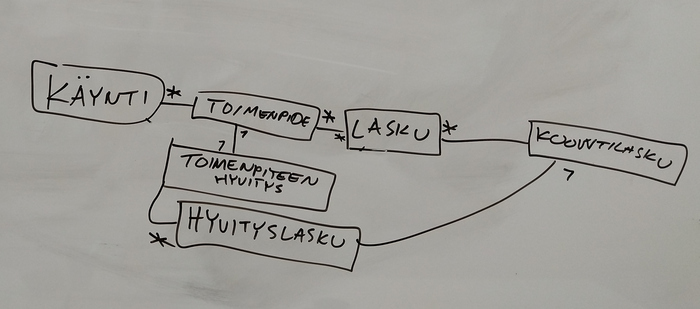
\includegraphics[width=\textwidth,height=0.3\textheight]{illustration/malli1.jpg}
\caption{\label{diarymalli1}: Ensimmäinen malli}
\end{figure}

Oikeastaan käynnillä voi olla monta erillistä asiaa, ne ovat
laskutettavia toimenpiteitä. Palaverin lopuksi aikaansaatu kaavio on
kuvassa \ref{diarymalli1}.

Tämä päätettiin toteuttaa.

Minulla meni torstaisen kokouksen jälkeen perjantai ja maanantai
perusrakenteen pystyttämiseen: Falcon, Ariadne GraphQL, Gunicorn ja
muutamia muita työkaluja. Lisäksi hommasin Pytest-testikirjaston, ja
opiskelin sen.

Lisäksi piti asentaa Apollo GraphQL-client ja Vue-cli, sekä plugin
Vue-Apollo.

Tiistaina sain ensimmäisen toiminnon, käyntien lisäämisen, valmiiksi.

Oli mielenkiintoista huomata, miten piirtämäni kuva ja tässä vaiheessa
aikaansaamani GraphQL-skeema muistuttivat läheisesti toisiaan.
GraphQL-queryjen sisältämät oliot rakensivat saman rakenteen, joka
tussitaululle piirsin. Sen sijaan GraphQL-mutaatioiden rooli ei ole
vielä auennut.

\hypertarget{viikko-2}{%
\section{Viikko 2}\label{viikko-2}}

Ensimmäisellä kehitykseen käyttämälläni viikolla (to-to) sain siis vain
ekan ominaisuuden valmiiksi. Sen jälkeen loppuviikosta tein vielä
käyntien laskutuksen. Lienee rehellistä arvioida, että noin viikon
kehitystyön myötä kaksi ``käyttäjätarinaa'' valmistui.

Perjantaina myös kirjoitin frontendia Vue-Apollolla ja käytin melkoisen
määrän aikaa kirjaston ominaisuuksien hahmottamiseen. Se ei kuulu
suoraan insinöörityön sisältöön, mutta toisaalta kuitenkin tarjoaa hyvän
kehyksen asioiden tekemiseen.

\hypertarget{viikko-3}{%
\section{Viikko 3}\label{viikko-3}}

Sain ensimmäisen version laskuhärvelistä valmiiksi. Tavoite oli Lauran
kanssa pitää asiasta palaveri perjantaina, mutta se peruuntui, koska
Laura oli tulossa kipeäksi.

Laskuhärveli toimii sinänsä, ja on hankala miettiä, onko siitä apua.

Kuitenkin domain-tason konseptien mallintaminen GraphQL-skeemaksi toimii
hyvin. Esimerkki, jossa koontilaskulla (ConsolidatedInvoice) voi olla
monta laskua (Invoice):

\begin{verbatim}
Type Invoice {
  number: Int
  sum: Float
  date: Date
}

type ConsolidatedInvoice {
  number: Int
  invoices: [Invoice]
}
\end{verbatim}

\hypertarget{palaveri-lauran-kanssa-tietomallin-kehittuxe4misestuxe4}{%
\section{27.9.2021 - Palaveri Lauran kanssa tietomallin
kehittämisestä}\label{palaveri-lauran-kanssa-tietomallin-kehittuxe4misestuxe4}}

Esittelin Lauralle tähän asti luomani softaproton. Pääasiallinen ongelma
on mielestäni laskun ja käynnin välisessä yhteydessä. Se, että laitetaan
käynti suoraan laskulle, on ongelmallista. Olin jo pitkin viikkoa
miettinyt, voisiko olla olemassa \textbf{Käyntirivi} ja \textbf{Käynnin
hyvitysrivi}, jotka sijaitsisivat laskulla ja koontilaskulla, ja
kumoaisivat toisensa.

Rupesin piirtämään Lauralle mallia, jossa Käynti liittyy Invoice-olioon,
ja Invoicea vastaa Credit Note, joka kumoaa Invoicella olevia käyntejä.
Piirsin Invoice- ja Credit note -olioiden sisään viivoja edustamaan
näitä käyntejä.

Laura totesi, että oikeastaan kirjanpidon kannalta täytyy täyttyä jokin
\textbf{Laskutusperuste}, jotta asia voidaan laskuttaa. Innostuin tästä
termistä, ja pyysin Lauraa jatkamaan. Laura sanoi, että laskutusperuste
on se, jonka pohjalta voidaan valita asioita laskutettavaksi. Asiat,
jotka täyttävät laskutusperusteen, mutta joihin ei liity laskua, voidaan
esimerkiksi listata laskuttamista varten. Pohjimmiltaan laskutusperuste
voi olla joko tavara tai palvelu, koska niitähän kaikki firmat myyvät.
Valitsimme laskutusperustetta kuvaamaan englanninkielisen termin
\textbf{BasisForInvoicing}. Palvelu on \textbf{Service}.

Ehdotin mallia, jossa \textbf{Appointment} voidaan viedä
\textbf{Invoicelle} \textbf{ServiceRow}-olioksi, jos täyttyy
BasisForInvoicing-ehto. Laura kurtisteli kulmiaan, eikä sanonut mitään.
Kysyin siis, eikö malli oikein miellytä, ja Laura totesi, että se
näyttää liian monimutkaiselta.

Pyyhin taulun puhtaaksi, ja kokeilimme uudestaan. Tein \textbf{Invoice}
-olion, jonka alle laitoin \textbf{ServiceRow} -nimisen olion. Invoicea
vastaamaan piirsin \textbf{CreditNote} -olion, jonka alle
\textbf{ServiceCreditRow}. Sivummas piirsin Appointment-olion, ja
pohdimme, mikä sen suhde voisi olla laskutukseen.

\begin{figure}
\centering
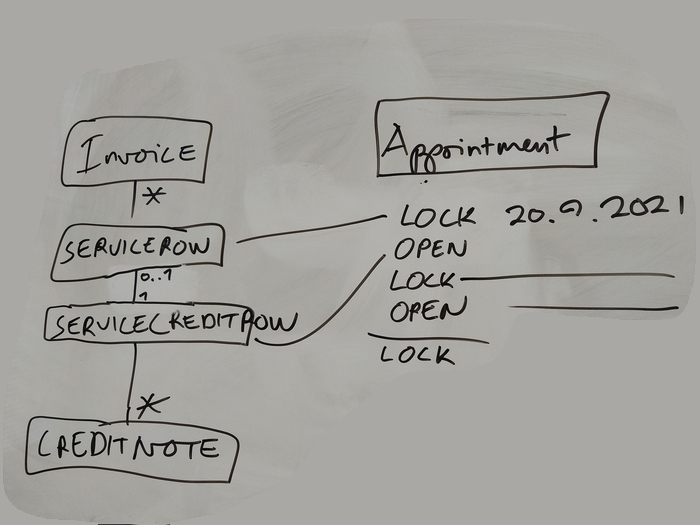
\includegraphics[width=\textwidth,height=0.5\textheight]{illustration/malli2.jpg}
\caption{\label{diarymalli2}Toinen malli}
\end{figure}

Yhtäkkiä minulla välähti: mitä, jos tehtäisiin ikäänkuin loki
\textbf{Appointment}-olion sisälle: sinne tallennettaisiin
lukitustapahtuma, kun \textbf{Appointment} liitetään laskulle luomalla
sitä vastaava \textbf{ServiceRow}. Ja vastaavasti kun
\textbf{ServiceRow} hyvitettäisiin \textbf{ServiceCreditRown} avulla,
voitaisiin luoda avaustapahtuma. Näin ollen \textbf{Appointment}-luokan
alla olisi lista tapahtumia, ja listan avulla nähtäisiin sekä
laskutushistoria, että myös käynnin tämänhetkinen laskutustilanne:
Laskuttamatta vai avoinna? Esitän mallin kuvassa \ref{diarymalli2}.

Laura huomautti, että tämä ei kuitenkaan ratkaise sitä pääongelmaa, joka
meillä on ollut: että käynnin hinta pitäisi jakaa monelle eri
maksajalle, joille lähetettyjä laskuja on voitava hyvittää itsenäisesti.

Niinpä pyyhin taas koko taulun puhtaaksi, ja lähdimme taas uudelleen
liikkeelle.

Nyt Käynnin alle lisättiin erillinen, laskutustarkoituksiin käytettävä
olio, jonka nimeksi pistettiin \textbf{BasisForInvoicing}. Tämä
BasisForInvoicing voidaan jakaa osiin, ja jokainen osa sisältää oman
erillisen listansa laskutustapahtumista: onko osa liitetty laskuun, vai
onko se hyvitetty ja taas siis avoinna.

\begin{figure}
\centering
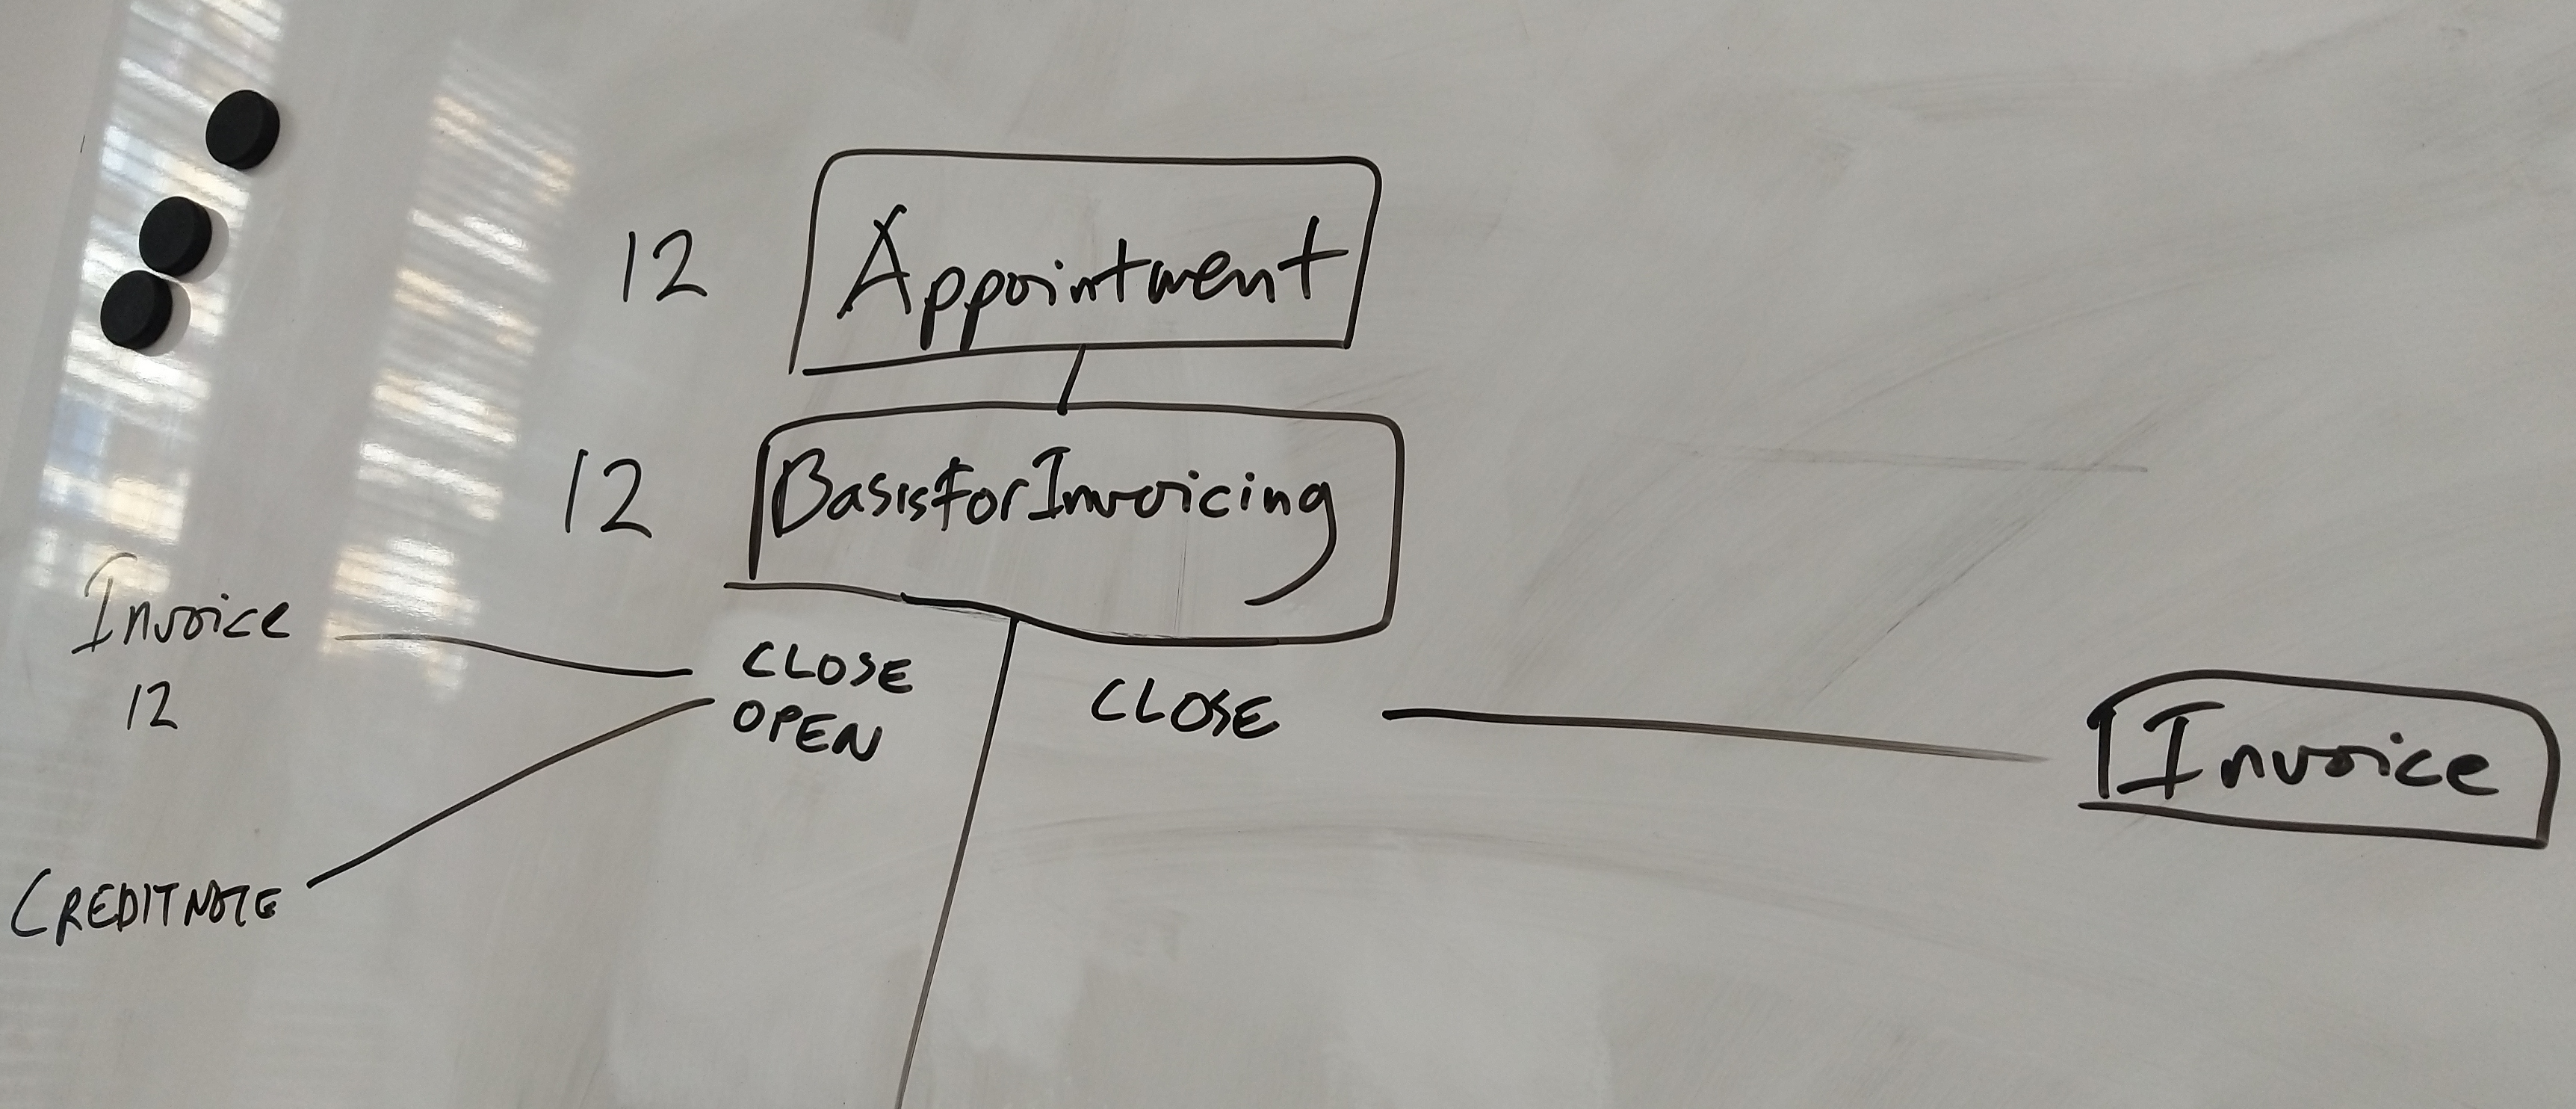
\includegraphics[width=\textwidth,height=0.5\textheight]{illustration/malli3.jpg}
\caption{\label{diarymalli3}Kolmas malli}
\end{figure}

Tämä tuntui meistä hyvältä mallilta, ja sen pohjalta ryhdyin koodaamaan.
Tätä mallia esittää kuva \ref{diarymalli3}. Sovittiin uusi palaveri
viikon päähän.

\hypertarget{viikko-4}{%
\section{Viikko 4}\label{viikko-4}}

Tiistai meni refaktoroidessa mallia uudelle tolalle, Lauran kanssa
keskustellun mukaisesti. Keskiviikkona taas toteutin ominaisuuden, jossa
laskut ja hyvityssummat täsmää. Torstain ja perjantain käytin rakentaen
uuden logiikan mukaista listausta käynneille ja laskuille: aiemmin
käyntejä käsitelleet laskuoliot piti nyt siirtää käyttämään
\textbf{Service-} ja \textbf{ServiceCredit}-olioita. Nämä vastaavat
käyntiä ja käynnin hyvitystä.

Lopulta tämä logiikka jäi sisällöllisesti aika kauas siitä, mitä Lauran
kanssa puhuttiin. Näin viikon lopulta katsottuna tuntuu, että olisi
pitänyt sopia selkeämmät tavoitteet myös sovelluksen toiminnan osalta:
mitä käyttäjätarinoita otetaan viikon ajaksi työn alle?

Positiivisena puolena taas on todettava, että malli syveni. Keskeinen
uusi löydös tässä on ketju \textbf{Appointment} -\textgreater{}
\textbf{Service} -\textgreater{} \textbf{ServiceCredit}. Nuolet kuvaavat
kulkusuuntaa, jossa rakennetta käydään läpi. Appointment siis tietää,
liittyykö siihen ``Service'' eli onko se jo laskutettu, ja Service taas
tietää, liittyykö siihen ServiceCredit.

\hypertarget{viikko-5}{%
\section{Viikko 5}\label{viikko-5}}

Maanantainen palaveri Lauran kanssa oli omasta mielestäni jotenkin
jähmeä. Epäilen, että osasyynä oli tussitaulullisen neukkarin puute.
Paras anti oli se, että päätettiin joukko tarinoita, joita teen
eteenpäin.

Ensimmäisenä lähdin toteuttamaan tarinaa, jossa jo kerran laskutettu
mutta hyvitetty käynti on voitava hyvittää uudelleen. Ratkaisin asian
tekemällä listan laskurivejä, jotka on liitetty käyntiin. Jos riviä
vastaa hyvitysrivi, on laskun summa taas avoinna. Tämä muistuttaa
aikaisempaa ideaani lokista, mutta on yksinkertaisempi: se perustuu
ServiceRow:n ja ServiceCreditin väliseen kytkökseen.

\hypertarget{viikko-6}{%
\section{Viikko 6}\label{viikko-6}}

Maanantain aloitin voimakkaalla refaktoroinnilla: tarvitaan SalesItem,
joka jakautuu SalesShareiksi, jotka puolestaan kytkeytyvät laskuilla
oleville SalesRow-olioihin.

Tämä vaatii isoja muutoksia alla olevaan mallin koodiin, ja siihen kului
koko maanantai. Olin aloittanut työn jo viime perhjantaina.
